\documentclass[12pt]{article}
\usepackage{amsmath}
\usepackage{amsfonts}
\usepackage{amssymb}
\usepackage{graphicx}
\usepackage[a4paper, margin=0.98in]{geometry}
\usepackage{physics}
\usepackage{float}
\usepackage{booktabs}
\usepackage{makecell}
\usepackage{helvet}
\usepackage{fancyhdr}
\usepackage{titling}
\usepackage{longtable}
\usepackage{caption}
\usepackage{enumitem}
\usepackage[american]{circuitikz}
\usepackage[hidelinks]{hyperref}
\usepackage{tikz}
\usepackage{subcaption}
\ctikzset{logic ports=ieee}





% Define header
\pagestyle{fancy}
\fancyhf{}
\fancyhead[R]{PH3204: Electronics Laboratory}

% Title
\title{
  \vspace{-2cm}
  \Huge \textbf{PH3204: Electronics Laboratory} \\[0.4cm]
  \Large \textbf{ Study of 555 Timer IC as Astable multivibrator with different frequency}
}

\author{
  \textbf{Ronit Bhuyan (22MS025)} \\[0.2cm]
  \textbf{Sub-Group B01}
}

\date{\today}

\begin{document}


\maketitle

\tableofcontents
\noindent\rule{\textwidth}{0.4pt}
\newpage

\section{Theory}
\subsection{554 Timer IC}
The 555 timer IC is a widely used integrated circuit designed to produce a variety of output waveforms and timing intervals. The name 555 comes from the fact that it contains three $5 k\omega$ rsistances in its internal structure. The 555 timer chip is a 8 pin robust device that can b configured in various modes such namely astable, bistable and multistabe modes. \\
A simplifoed block diagram of the 555 timer is shown in the figure \ref{fig:555_timer}
\begin{figure}[H]
   \centering
    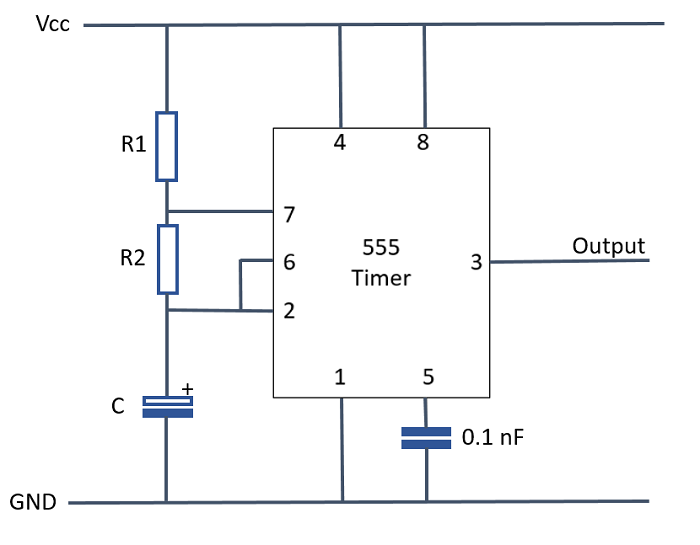
\includegraphics[width=0.5\textwidth]{"D:/ronit/IISER-K/6 SEM/PH3204/Reports/exp05/EN555-circuit-diagram-astable-mode.png"}
    \caption{555 timer IC}
    \label{fig:555_timer}
\end{figure}
\noindent
The various pin functions are stated below:
\begin{itemize}
    \item \textbf{Pin 1 (GND)}: Ground pin. This pin is connected to the negative terminal of the power supply.
    \item \textbf{Pin 2 (TRIG)}: Trigger pin. This pin is used to trigger the timer and initiate the timing cycle. A negative pulse on this pin starts the timing interval.
    \item \textbf{Pin 3 (OUT)}: Output pin. This pin provides the output signal of the timer. It can sink or source current to drive external loads.
    \item \textbf{Pin 4 (RESET)}: Reset pin. This pin is used to reset the timer and terminate the timing cycle. A low signal on this pin resets the output to low.
    \item \textbf{Pin 5 (CTRL)}: Control voltage pin. This pin is used to control the timing interval by applying an external voltage. It is typically connected to ground through a capacitor to filter noise.
    \item \textbf{Pin 6 (THRESH)}: Threshold pin. This pin is used to monitor the voltage across the timing capacitor. When the voltage on this pin exceeds 2/3 of the supply voltage, the timer resets.
    \item \textbf{Pin 7 (DISCH)}: Discharge pin. This pin is used to discharge the timing capacitor when the timer is in the astable or monostable mode. It is connected to ground when the timer is in the timing cycle.   
    \item \textbf{Pin 8 (VCC)}: Supply voltage pin. This pin is connected to the positive terminal of the power supply. The supply voltage can range from 4.5V to 15V.
\end{itemize} 

\subsection{Astable Multivibrator}
An astable multivibrator is a type of oscillator circuit that continuously switches between its high and low states without requiring any external triggering. The 555 timer can be configured as an astable multivibrator by connecting resistors and capacitors in a specific manner. In this configuration, the 555 timer generates a square wave output signal with a frequency determined by the values of the resistors and capacitor used in the circuit.\\
The output frequency of the astable is given by the formula:
\begin{equation}
    f = \frac{1.44}{(R_1 + 2R_2)C_1}
\end{equation}
where $R_1$ and $R_2$ are the resistances in $\Omega$ and $C_1$ is the capacitance in Farads.\\


\section{Data and Observations}
We havve chosen different values of $\mathrm{R_1}$ $\mathrm{R_2}$ and $\mathrm{C_1}$ to observe the frequency of the output signal. Using these values we have calculated the theoretical frequency values using the formula given above.\\
Using the oscilloscope, we measured the time-period of the output wave generated to calculate its frequency and compared it with the theoretical calculations. \\
The data collected has been tabulated below.
\begin{longtable}{|c|c|c|c||c|c|c|c||c|}
    \hline
    $\mathrm{C_1\ (nF)}$ & $\mathrm{R_1\ (k\Omega)}$ & $\mathrm{R_2\ (k\Omega)}$ & $f_\mathrm{th}\ (\mathrm{kHz})$ & $T_m\ (\mu s)$ & $T_s\ (\mu s)$ & $T\ (\mu s)$ & $f_\mathrm{exp}\ (\mathrm{kHz})$ & \% Error \\
    \hline
    \endfirsthead
    
    \hline
    $\mathrm{C_1\ (nF)}$ & $\mathrm{R_1\ (k\Omega)}$ & $\mathrm{R_2\ (k\Omega)}$ & $f_\mathrm{th}\ (\mathrm{kHz})$ & $T_m\ (\mu s)$ & $T_s\ (\mu s)$ & $T\ (\mu s)$ & $f_\mathrm{exp}\ (\mathrm{kHz})$ & \% Error \\
    \hline
    \endhead
    
    \hline
    \endfoot
    
    \endlastfoot
    
    1 & 1.01 & 10.25 & 65.0860 & 8.12 & 7.34 & 15.46 & 64.6831 & 0.62 \\ \hline
    1 & 10 & 100 & 6.6667 & 72.4 & 65.6 & 138 & 7.2464 & 8.71 \\ \hline
    1 & 100 & 1000 & 0.6667 & 724 & 644 & 1368 & 0.7310 & 9.65 \\ \hline
    10 & 1 & 10 & 6.6667 & 74.8 & 72.4 & 147.2 & 6.7935 & 1.90 \\ \hline
    10 & 10 & 100 & 0.6667 & 768 & 704 & 1472 & 0.6793 & 1.89 \\ \hline
    10 & 100 & 1000 & 0.0667 & 8080 & 7520 & 15600 & 0.0641 & 3.85 \\ \hline
    100 & 1 & 10 & 0.6667 & 904 & 924 & 1828 & 0.5470 & 17.97 \\ \hline
    100 & 10 & 100 & 0.0667 & 9700 & 9000 & 18700 & 0.0535 & 19.78 \\ \hline
    100 & 100 & 1000 & 0.0067 & 96000 & 102000 & 198000 & 0.0051 & 24.24 \\ \hline
    0.1 & 100 & 1000 & 6.6667 & 96 & 82 & 178 & 5.6180 & 15.72 \\ \hline
    0.1 & 10 & 100 & 66.6667 & 8.8 & 8.2 & 17 & 58.8235 & 11.76 \\ \hline
    0.1 & 1 & 10 & 666.6667 & 2.6 & 1.6 & 4.2 & 238.0952 & 64.29 \\ \hline
    
    \caption{Table for frequency calculation}
\end{longtable}
\noindent
The above table shows except 1 outlier, the experimental and theoretical obervations matched pretty. Note that on last 6 observations were calculated on a different day and the oscilloscope was showing a lot of noise which made the calculations of the time period and hence frequency difficult. This could have given rise to more errors in the last 6 observations as compared to the first 6.\\
\\

\section{Sources of Error}
The possible sources of error in this experiment have been listed below:
\begin{itemize}
  \item The values of the resistors and capacitors used in this experiment may not be exact. This may affect the theoretical values of the frequency which in turn affects the error estimates.
  \item While measuring the time period through the oscilloscope, there were many cases where it showed a lot of noise, which made the accurate calculation of time period and frequency difficult. This could also lead to some errors in the experimental values of the frequency.
  \item Finally, observed values could be affected due to faulty instruments or loose connections.
\end{itemize}

\section{Conclusion}
In this experiment, we successfully studied the 555 timer IC in the astable mode. We observed the square waves and calculated the output frequency using the oscilloscope. This experimentally determined value was compared to the theoretical value.The experimental results were found to be close to the theoretical values except for a specific case.

\end{document}